\chapter{Ecuación de onda}
\label{cap:wave}
\begin{resumen}
	En este capítulo desarrollaremos dos métodos numéricos, basados en las diferencias finitas, para aproximar la solución a la ecuación de onda en una  y dos dimensiones.
\end{resumen}

\section{Caso lineal}
Tenemos la siguiente ecuación:
\begin{equation}
	\label{eq:1dwaveeq}
	\frac{\partial^2u}{\partial t^2} - c^2\frac{\partial^2u}{\partial x^2} = 0
\end{equation}
a la que le pediremos las condiciones iniciales
\begin{equation}
	\label{eq:1dwaveini}
\begin{cases}
	u(x,0) = f(x) \hspace{15px} -\infty < x < \infty \\
	\frac{\partial u(x,0)}{\partial t} = g(x) \hspace{15px} -\infty < x < \infty 
\end{cases}
\end{equation}
Como es costumbre, lo primero que tenemos que hacer es probar la existencia y unicidad de la solución antes de aproximarla
\subsection[Existencia y unicidad]{Existencia y unicidad\footnote{Esta demostración puede encontrarse en el artículo de \cite{1dwavedem}}}
Si hacemos el cambio de variable $\xi = x-ct, \hspace{5px} \eta = x+ct$. Aplicando la regla de la cadena, obtenemos
\begin{equation*}
	\frac{\partial}{\partial x} = \frac{\partial\xi}{\partial x}\frac{\partial}{\partial\xi} + \frac{\partial\eta}{\partial x}\frac{\partial}{\partial\eta} = \frac{\partial}{\partial\xi} + \frac{\partial}{\partial\eta}
\end{equation*}
y
\begin{equation*}
	\frac{\partial}{\partial t} = \frac{\partial\xi}{\partial t}\frac{\partial}{\partial\xi} + \frac{\partial\eta}{\partial t}\frac{\partial}{\partial\eta} = -c\frac{\partial}{\partial\xi} +c \frac{\partial}{\partial\eta}
\end{equation*}

Luego, si sustituimos en la ecuación \ref{eq:1dwaveeq} con las igualdades anteriores, obtenemos que una función es solución de \ref{eq:1dwaveeq} si y solo sí cumple
\begin{equation*}
	\frac{\partial^2 u}{\partial\xi\partial\eta} = 0
\end{equation*}
Es trivial (integrando dos veces) observar que esta la solución a esta última ecuación será de la forma
\begin{equation}
	\label{eq:1dwave2}
	u(x,t) = P(\xi) + Q(\eta) = P(x-ct) + Q(x+ct)
\end{equation}
para unas funciones $P$ y $Q$ arbitrarias.
Ahora, si utilizamos las condiciones iniciales \ref{eq:1dwaveini} tenemos las relaciones
\begin{equation*}
	P(x) + Q(x) = f(x), \hspace{20px} P'(x) - Q'(x) = \frac{1}{c}g(x). 
\end{equation*}
Ahora, si integramos la segunda relación en el intervalo $[0,x]$, y la sumamos y restamos a la primera y definimos $K=\frac{1}{2}[P(0)-Q(0)]$, obtenemos cómo son las funciones
\begin{equation*}
	P(x) = \frac{1}{2}f(x) + \frac{1}{2c}\int_{0}^{x}g(\zeta)d\zeta + K
\end{equation*}
\begin{equation*}
	Q(x) = \frac{1}{2}f(x) - \frac{1}{2c}\int_{0}^{x}g(\zeta)d\zeta - K
\end{equation*}
Luego, simplemente sustituyendo en \ref{eq:1dwave2}, obtenemos que
\begin{equation}
	\label{eq:1dwavesol}
	u(x,t) = \frac{1}{2}[f(x+ct)+f(x-ct)] + \frac{1}{2c}\int_{x-ct}^{x+ct}g(\zeta)d\zeta.
\end{equation}
\begin{teorema}[Existencia y unicidad]
	Si $f$ y $g$ son funciones integrables, la ecuación \ref{eq:1dwaveeq} con los valores iniciales \ref{eq:1dwaveini} tiene solución y además esta es única.
\end{teorema}
\begin{proof}
 	La función definida en \ref{eq:1dwavesol} es, por construcción, solución de la ecuación diferencial, luego la existencia está demostrada.
 	Demostrar la unicidad es sencillo, pues si suponemos que $v(x,t)$ es solución de \ref{eq:1dwaveeq}, llegamos a la conclusión de que tiene que ser de la forma \ref{eq:1dwavesol}, ya que todos los argumentos hechos en esta subsección son reversibles. 
\end{proof}

\subsection[Aproximación de la solución]{Aproximación de la solución\footnote{Las demostraciones de toda esta sección son modificaciones propias de \cite{anummeth}}}

Utilizando la notación descrita en la sección \ref{sec:notacion}, aproximaremos la ecuación \ref{eq:1dwaveeq} por el cociente incremental 

\begin{equation*}
	\begin{split}
	u_{t\bar t}(x,t) - c^2u_{x\bar{x}}(x,t) = 0 \Rightarrow \frac{1}{\Delta t^2}[u(x,t + \Delta t)-2u(x,t)+u(x, t - \Delta t)]  = \\ \left(\frac{c}{\Delta x}\right)^2[u(x+\Delta x,t)-2u(x,t)+u(x-\Delta x, t)]
	\end{split}
\end{equation*}

Si ahora nos ceñimos a la malla de puntos de la que hablamos en \ref{sec:notacion}, tenemos
\begin{equation*}
	\begin{split}
	\frac{1}{\Delta t^2}[u_{i,j+1}-2u_{i,j}+u_{i,j-1}] = \left(\frac{c}{\Delta x}\right)^2[u_{i+1,j}-2_{i,j}+u_{i-1,j}] \Rightarrow \\
	u_{i,j+1} = \left(c\frac{\Delta t}{\Delta x}\right)^2[u_{i+1,j}-2u_{i,j}+u_{i-1,j}] + 2u_{i,j} - u_{i,j-1}	
	\end{split}
\end{equation*}
Lo que, tras combinar elementos, nos queda en
\begin{equation}
	\label{eq:1dwave_formula}
	u_{i,j+1} =  2\left[1 - \left(c\frac{\Delta t}{\Delta x}\right)^2\right]u_{i,j} + \left(c\frac{\Delta t}{\Delta x}\right)^2[u_{i+1,j} + u_{i-1,j}] - u_{i,j-1}.
\end{equation}


\begin{figure}[h]
	\centering
	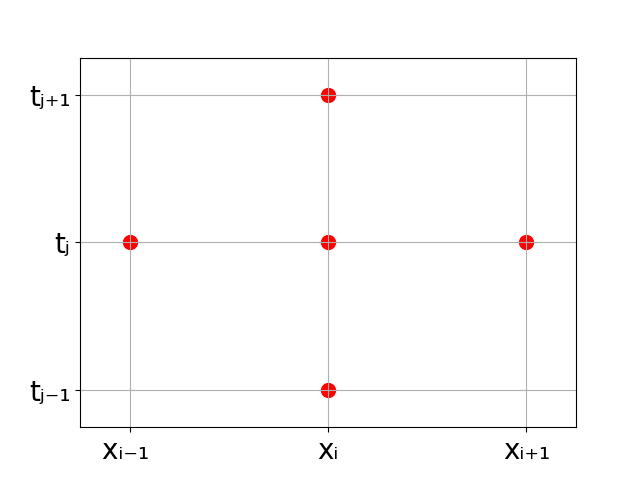
\includegraphics[scale=0.5]{./Imagenes/Bitmap/1dwave.png}
	\caption{Representación en la malla del esquema \ref{eq:1dwave_formula}}
\end{figure}

Esto indica que, para calcular $u_{i,j}$ para cualquier tiempo $j\in\mathbb{N}$ necesitamos conocer el valor de la función en los dos tiempos anteriores. Esto no será un problema, pues los valores para $u(x,0) = f(x)$ por el problema del valor inicial.

Calcular los valores para $t=\Delta t$ tampoco es difícil, pues $u(x,\Delta t) \equiv u(x,0) + \Delta t u_t(x,0) \equiv f(x) +\Delta tg(x)$.

Si definimos $\lambda = c\frac{\Delta t}{\Delta x}$, la convergencia del esquema numérico depende exclusivamente de su valor. Si $\lambda > 1$, el método diverge \footnote{Esto no lo probaremos, pero puede encontrarse una demostración en \citet{anummeth}, p. 487.}. Por otro lado, si $\lambda <=1$, el esquema converge.

Lo probaremos solo para $\lambda=1$ (que es el caso que usaremos), pero puede encontrarse en \citet{anummeth} una demostración para $0<\lambda<=1$.

\begin{teorema}
	Si $\lambda=1$ y $f,g\in\mathscr{C}^2(\mathbb{R})$, la aproximación dada por \ref{eq:1dwave_formula} converge a la solución de \ref{eq:1dwaveeq} cuando $\Delta x = c\Delta t \longrightarrow 0$.
\end{teorema}
\begin{proof}
	Primero definimos el siguiente valor.
	\begin{equation*}
		D_{i,j} := u_{i,j} - u_{i-1,j-1} \hspace{20px} \forall 1<=j.
	\end{equation*}
	Ahora, como $\lambda = 1$ podemos rescribir la ecuación \ref{eq:1dwave_formula} como 
	\begin{equation*}
		u_{i,j+1} - u_{i-1,j} = u_{i+1,j} - u_{i,j-1} \Rightarrow D_{i,j+1} = D_{i+1,j}.
	\end{equation*}
	Aplicando ahora esa fórmula de manera recursiva, podemos observar la siguiente relación
	\begin{equation}
		\label{aux}
		D_{i,j+1} = D_{i+k,j-k+1} \hspace{20px} \forall 0<=k<=j.
	\end{equation}
	Además, por como ha sido definido $D$, es fácil observar que para cualesquiera $i,j$, se tiene que
	\begin{equation*}
		\sum_{k=0}^{j}D_{i-k,j-k+1} = u_{i,j+1} - u_{i-j-1,0}
	\end{equation*}
	Despejando en la última ecuación podemos obtener la fórmula explícita
	\begin{equation*}
		u_{i,j+1} = u_{i-j-1,0} + \sum_{k=0}^{j}D_{i-k,j-k+1}
	\end{equation*}
	Pero, primero teniendo en cuenta que $u_{i-j-1,0}=f_{i-j-1}$, y gracias a \ref{aux}, podemos sustituir los sumandos del sumatorio por términos más simples, y obtener
	\begin{equation*}
		u_{i,j+1} = f_{i-j-1} + \sum_{k=0}^{j}D_{i+j-2k,1} = f_{i-j-1} + \sum_{k=0}^{j}(u_{i+j-2k,1} - u_{i+j-2k-1,0})
	\end{equation*}
	Por otro lado, ya vimos que $u_{i,1} = f_i + \Delta tg_i$, luego en última instancia, la ecuación se nos queda como
	\begin{equation}
		\label{aux2}
		u_{i,j+1} = f_{i-j-1} + \Delta t\sum_{k=0}^{j}g_{i+j-2k} + \sum_{k=0}^{j}(f_{i+j-2k}-f_{i+j-2k-1})
	\end{equation}
	Como $t_n=n\Delta t$, se tiene que $x_n=n\Delta x=nc\Delta t=ct_{n}$, por ello, para cualquier función $F$ se tiene que $F_{i+j}:=F(x_{i+j})=F(x_i+ct_j)$.
	
	Como $f$ tiene derivada continua, usando el teorema del valor medio obtenemos que $\exists\theta_k\in(-1,0)$ tal que
	\begin{equation*}
		f_{i+j-2k}-f_{i+j-2k-1} = f(x_{i-2k}+ct_j) - f(x_{i-2k}+ct_{j}-\Delta x) = \Delta xf'(x_{i-2k}+ct_j+\theta_k\Delta x).
	\end{equation*} 
	Además, $f_{i-j-1}=f(x_{i-j-1})=f(x_i-(j+1)\Delta x)=f(x_i -(j+1)c\Delta t)=f(x_i-ct_{j+1})$. Haciendo algo muy similar, obtenemos las igualdades $g_{i+j-2k}=g(x_i+ct_{j+1}-[2k+1]\Delta x)$ y $f'(x_{i-2k}+ct_j+\theta_k\Delta x)=f'(x_i+ct_{j+1}+\theta_k\Delta x - [2k+1]\Delta x)$
	
	Sean x,t fijos hagamos tender $\delta x=c\Delta t$ a 0, y $i,j$ tender a infinito de manera que se mantengan las relaciones $x_i=x$ y $t_j+1=t$ siempre.
	Si sustituimos en \ref{aux2} con todas las igualdades que hemos obtenido, tendremos
	\begin{equation*}
	\begin{split}
		u_{i,j} = f(x_i-ct_{j+1}) + \frac{1}{2c}\sum_{k=0}^{j}2\Delta xg(x_i+ct_{j+1}-[2k+1]\Delta x) + \\ \frac{1}{2}\sum_{k=0}^{j}2\Delta xf'(x_i+ct_{j+1} +\theta_k\Delta x - [2k+1]\Delta x)
	\end{split}
	\end{equation*}
	Que, pasando al límite se nos queda en
	\begin{equation*}
	\begin{split}
		u_{i,j} = f(x_i-ct_{j+1}) + \frac{1}{2c}\lim_{\Delta x\rightarrow0}\sum_{k=0}^{j}2\Delta xg(x_i+ct_{j+1}-[2k+1]\Delta x) + \\ \frac{1}{2}\lim_{\Delta x\rightarrow0}\sum_{k=0}^{j}2\Delta xf'(x_i+ct_{j+1} +\theta_k\Delta x - [2k+1]\Delta x) =^{*} \\
		f(x-ct) + \frac{1}{2c}\int_{0}^{2ct}g(x+ct-\xi)d\xi + \frac{1}{2}\int_{0}^{2ct}f'(x+ct-\xi)d\xi
	\end{split}
	\end{equation*}
	\com{La igualdad que tiene un asterisco la he copiado del libro y no la entiendo. Entiendo conceptualmente que al pasar al límite de un sumatorio estamos haciendo una integral y que el diferencial es "lo que se hace pequeño en el límite", pero no sé el formalismo matemático que se ha aplicado.
		
	Además hay otro problema, aun suponiendo eso que no entiendo, las integrales me dan \textit{casi} los resultados que necesito. Como no sé de dónde ha salido la última igualdad, no puedo comprobar si hay alguna pequeña errata.

	En cualquier caso supondré que he terminado la demostración}
	
	Pero el final de la última serie de igualdades es exactamente \ref{eq:1dwavesol}, luego hemos demostrado que la aproximación tiende a la solución exacta de la ecuación.
\end{proof}

\section{Caso bidimensional}


